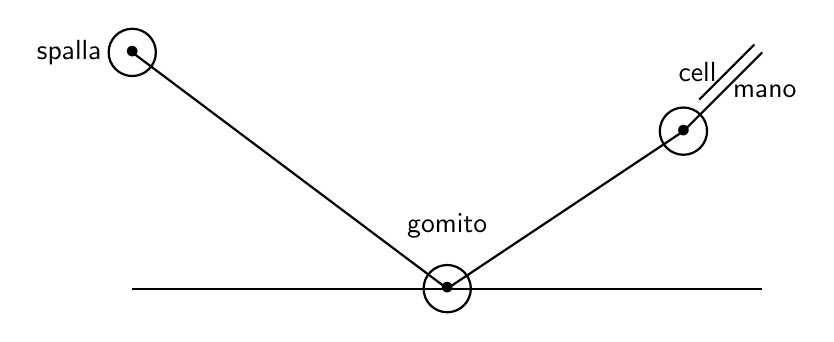
\begin{tikzpicture}[%
molla/.style={decorate,decoration={snake,post length=5,amplitude=5,pre length=5,segment length=5}, thick},
thick%
]
\sffamily \sansmath
%	\draw [help lines] (0, 0) grid (8, 5);
	
	\draw (8, 0) -- (0, 0);
	
	\draw (0, 3) circle (0.3)
		node at (0, 3) {$\bullet$};
	\node [] at (-.8, 3) {spalla};
	\draw (0, 3) -- (4, 0);
	\draw (4, 0) circle (0.3)
		node {$\bullet$};
	\node [] at (4, 0.8) {gomito};
	\draw (4, 0) -- (7, 2);
	\draw (7, 2) circle (0.3)
		node {$\bullet$};
	\draw (7, 2) -- (8, 3)
		node [pos=0.5, right] {mano};
	\draw (7.2, 2.4) -- (7.9, 3.1)
		node [pos=0.5, left] {cell};

  \end{tikzpicture}